\section{Matriz de tiempos de residencia} \label{res:matriz}

En esta sección se muestra la matriz de tiempos de residencia que se usará en las simulaciones. En primer lugar se mostrarán los resultados obtenidos a partir del algoritmo \ref{alg:timematrix}, los que permitirán tener una idea del comportamiento de las personas de la ciudad de Santiago en condiciones normales.

Primero se estudiarán los resultados obtenidos con una lista de ambientes extensiva, que incluye prácticamente todos los propósitos listados por la Encuesta Origen Destino. Con respecto a las clases, se utiliza una clasificación por edad, sexo y nivel dde ingresos. Esto entrega una matriz de 18 clases y 13 ambientes que refleja el comportamiento pre-pandeamia de los santiaguinos.

Como se discutió en \ref{met:decisiones}, esta matriz es demasiado granular y no hay datos suficientes para actualizarla con el comportamiento durante la pandemia. Por tanto, en segundo lugar se mostrará la matriz definitiva a utilizar en las simulaciones, la cual solo tiene 5 clases y 2 ambientes.

En segundo lugar, se mostrarán los datos de movilidad para los distintos grupos, y la matriz a tiempo variable. Esto nos dará una idea del comportamiento a lo largo de la pandemia. 

\subsection{Santiago en condiciones normales}

% El código para esta sección esta en el github...
El código para esta sección se encuentra en el repositorio de GitHub \textit{tabitaCatalan/lagrangian-time}, específicamente en el directorio \texttt{src/time\_residence\_matrix/}.\\


\noindent \textbf{Matriz detallada}\\
% Elección de clases y ambientes, lista de ambientes disponibles en la EOD, cómo se eligieron las clases, etc. Esto debería estar docuementado en el repo. 
% \ref{alg:timematrix} 
Para evaluar los resultados del algoritmo, se aplica a la Encuesta Origen Destino Santiago 2012, ya descrita en \ref{}. Las clases son elegidas combinando los tres criterios de la tabla \ref{table:clases-full}. El nivel socioeconómico es calculado en base a los datos de ingreso de cada persona provistos por la encuesta, agrupando a nivel de hogar y dividiendo por la cantidad de habitantes del hogar. Los ingresos de corte son elegidos de tal forma que cada tramo socioeconómico tiene unas \(20\,000\) personas.

\begin{table}[h!]
\centering
\begin{tabular}{||r|c||c||r|c||} 
 \hline
 \multicolumn{2}{||c||}{Edad (años)} & Sexo      & \multicolumn{2}{c||}{\begin{tabular}{@{}c@{}}Nivel Socioeconómico \\ (ingreso per cápita)\end{tabular}} \\
 \hline
 \textbf{Joven} & 0-24   & Hombre    & \textbf{Bajo}&\(\leq\) \$\(111\,666\)\\
 \textbf{Adulto} & 25-64 & Mujer     & \textbf{Medio}& \$ \(111\,667\) - \$ \(199\,999 \)\\
 \textbf{Mayor} & 65 o más &         & \textbf{Alto}&\(\geq\) \$ \(200\,000\)\\
 \hline
\end{tabular}
\caption{Criterios usados para obtener las clases de la matriz detallada a partir de la EOD2012 Santiago.}
\label{table:clases-full}
\end{table}


Los ambientes utilizados están basados en la lista de propósitos de viajes y los modos de transporte usados. Son los siguientes: \texttt{hogar}, \texttt{trabajo}, \texttt{estudios}, \texttt{compras}, \texttt{visitas}, \texttt{salud}, \texttt{trámites}, \texttt{recreación}, \texttt{transporte público}, \texttt{auto}, \texttt{caminata}, \texttt{bicicleta} y \texttt{otros}. La lista de propósitos de viajes y sus ambientes asociados se encuentra en la tabla \ref{table:ambientes-prop-full}. La lista de modos está en la tabla \ref{table:ambientes-modo-full}.

% \begin{table}[h!]
% \centering
% \begin{tabular}{||l|c||l|c||} 
%  \hline
%  \multicolumn{2}{||c||}{Propósito de viaje} &  \multicolumn{2}{c||}{Modo de transporte} \\
%  \hline
% 1. Al trabajo               & \texttt{trabajo}      & 1:Auto                        & \texttt{auto}\\
% 2. Por trabajo              & \texttt{trabajo}      & 2:Bus TS                      & \texttt{transporte público}\\
% 3. Al estudio               & \texttt{estudios}     & 3:Bus no TS                   & \texttt{transporte público}\\
% 4. Por estudio              & \texttt{estudios}     & 4:Metro                       & \texttt{transporte público}\\
% 5. De salud                 & \texttt{salud}        & 5:Taxi Colectivo              & \texttt{transporte público}\\
% 6. Visitar a alguien        & \texttt{visitas}      & 6:Taxi                        & \texttt{auto}\\
% 7. Volver a casa            & \texttt{hogar}        & 7:Bus TS - Bus no TS          & \texttt{transporte público}\\
% 8. Buscar o dejar a alguien & \texttt{visitas}      & 8:Auto - Metro                & \texttt{transporte público}\\
% 9. Comer o tomar algo       & \texttt{compras}      & 9:Bus TS - Metro              & \texttt{transporte público}\\
% 10.Buscar o dejar algo      & \texttt{compras}      & 10:Bus no TS - Metro          & \texttt{transporte público}\\
% 11.De compras               & \texttt{compras}      & 11:Taxi Colectivo - Metro     & \texttt{transporte público}\\
% 12.Tramites                 & \texttt{trámites}     & 12:Taxi - Metro               & \texttt{transporte público}\\
% 13.Recreación               & \texttt{recreación}   & 13:Otros - Metro              & \texttt{transporte público}\\
% 14.Otra actividad           & \texttt{otros}        & 14:Otros - Bus TS             & \texttt{transporte público}\\
%                             &                       & 15:Otros - Bus TS - Metro     & \texttt{transporte público}\\
%                             &                       & 16:Otros                      & \texttt{otros}\\
%                             &                       & 17:Caminata                   & \texttt{caminata}\\
%                             &                       & 18:Bicicleta                  & \texttt{bicicleta}\\
%  \hline
% \end{tabular}
% \caption{Propósitos de viaje y modos de transporte de la EOD2012, y sus ambientes asociados.}
% \label{table:ambientes-full}
% \end{table}

\begin{table}[h!]
\centering
\begin{tabular}{||l|c||} 
 \hline
 \multicolumn{2}{||c||}{Propósito de viaje} \\
 \hline
1. Al trabajo               & \texttt{trabajo}      \\
2. Por trabajo              & \texttt{trabajo}      \\
3. Al estudio               & \texttt{estudios}     \\
4. Por estudio              & \texttt{estudios}     \\
5. De salud                 & \texttt{salud}        \\
6. Visitar a alguien        & \texttt{visitas}      \\
7. Volver a casa            & \texttt{hogar}        \\
8. Buscar o dejar a alguien & \texttt{visitas}      \\
9. Comer o tomar algo       & \texttt{compras}      \\
10.Buscar o dejar algo      & \texttt{compras}      \\
11.De compras               & \texttt{compras}      \\
12.Tramites                 & \texttt{trámites}     \\
13.Recreación               & \texttt{recreación}   \\
14.Otra actividad           & \texttt{otros}        \\
 \hline
\end{tabular}
\caption{Propósitos de viaje de la EOD2012 y sus ambientes asociados.}
\label{table:ambientes-prop-full}
\end{table}

\begin{table}[h!]
\centering
\begin{tabular}{||l|c||} 
 \hline
 \multicolumn{2}{||c||}{Modo de transporte} \\
 \hline
 1:Auto                        & \texttt{auto}\\
 2:Bus TS                      & \texttt{transporte público}\\
 3:Bus no TS                   & \texttt{transporte público}\\
 4:Metro                       & \texttt{transporte público}\\
 5:Taxi Colectivo              & \texttt{transporte público}\\
 6:Taxi                        & \texttt{auto}\\
 7:Bus TS - Bus no TS          & \texttt{transporte público}\\
 8:Auto - Metro                & \texttt{transporte público}\\
 9:Bus TS - Metro              & \texttt{transporte público}\\
 10:Bus no TS - Metro          & \texttt{transporte público}\\
 11:Taxi Colectivo - Metro     & \texttt{transporte público}\\
 12:Taxi - Metro               & \texttt{transporte público}\\
 13:Otros - Metro              & \texttt{transporte público}\\
 14:Otros - Bus TS             & \texttt{transporte público}\\
 15:Otros - Bus TS - Metro     & \texttt{transporte público}\\
 16:Otros                      & \texttt{otros}\\
 17:Caminata                   & \texttt{caminata}\\
 18:Bicicleta                  & \texttt{bicicleta}\\
 \hline
\end{tabular}
\caption{Modos de transporte de la EOD2012 y sus ambientes asociados.}
\label{table:ambientes-modo-full}
\end{table}

La matriz obtenida \ref{img:Pmatrix-full} refleja el comportamiento esperado de la población de Santiago. Como era de esperarse, se pasa la mayor parte del tiempo en el hogar (de hecho, se redujo el tiempo en el hogar en 7 horas de tiempo de sueño). 

Algunas observaciones: los adultos pasan una cantidad considerable de tiempo en el trabajo, en especial los hombres. Los jóvenes pasan mucho tiempo en el ambiente estudios, especialmente los de clase alta; los jóvenes con menos ingresos pasan más tiempo en el trabajo. Los adultos mayores pasan mucho más tiempo en el hogar, pero los hombres pasan una cantidad importante de tiempo en el trabajo. 

El nivel socioeconómico medio pasa menos tiempo de compras y de visita que los demás. El auto es bastante más utilizado por la clase alta y por los adultos hombres de clase media. Los adultos mayores pasan más tiempo en el ambiente salud, especialmente los de clase baja.

En general los resultados son los esperados para una ciudad con una segregación importante como lo es Santiago. Es posible que en la última década se hayan reducido las diferencias de género, pero eso queda fuera del alcance de este trabajo.


\begin{figure}[h]
\centering
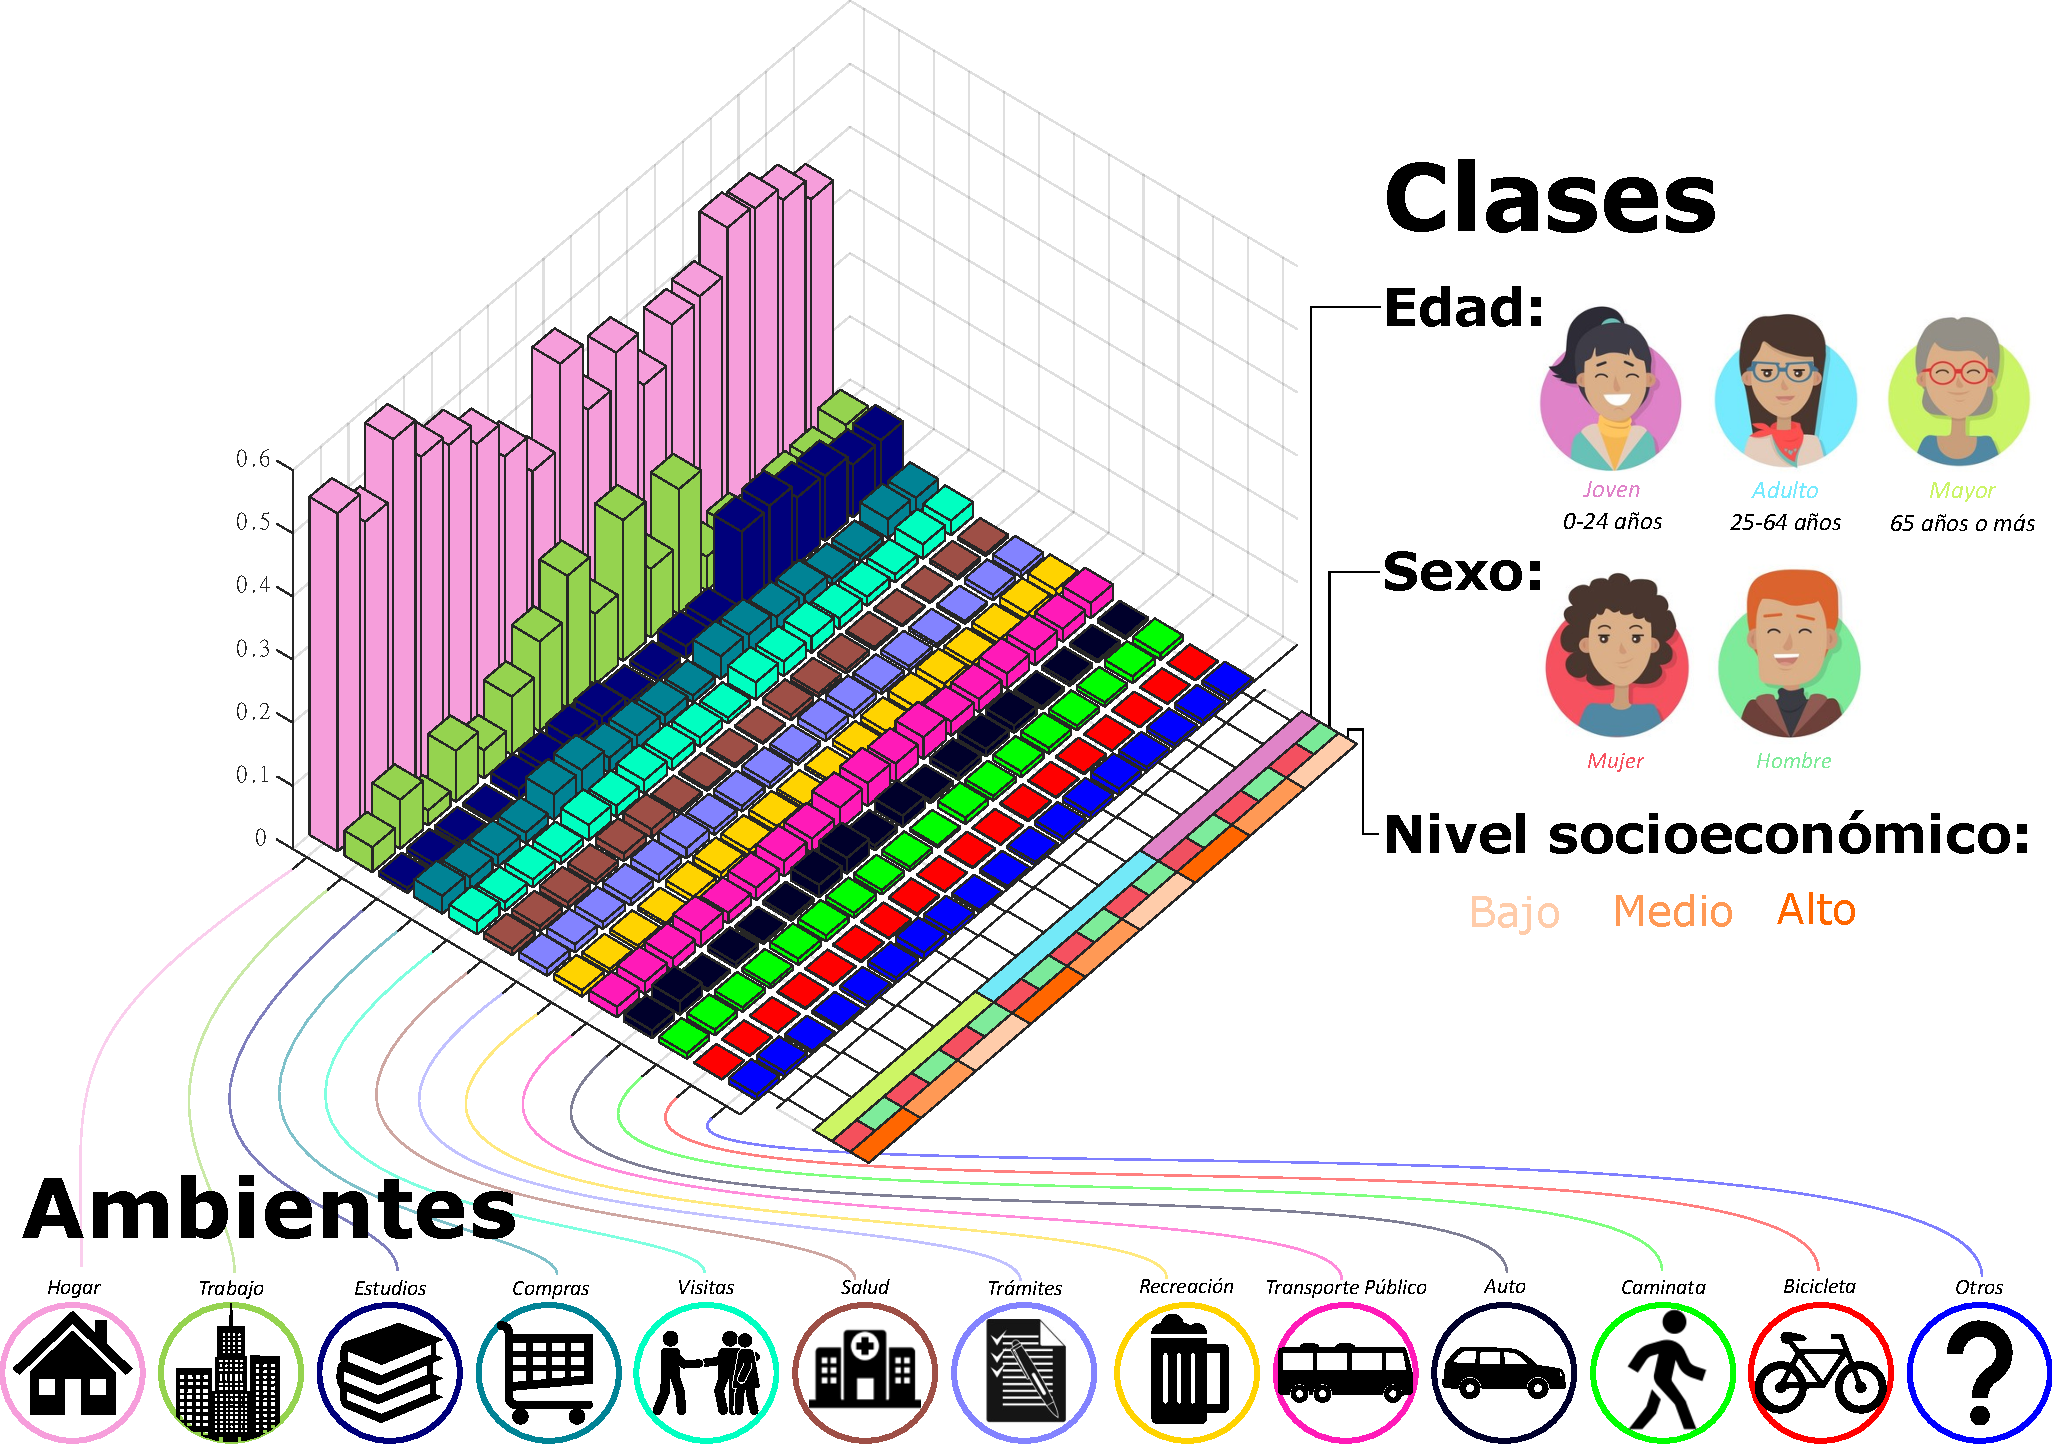
\includegraphics[width=0.99\textwidth]{img/resultados/matrixP/matriz Pambientesyclases.pdf}
\caption[Matriz detallada de tiempos de residencia para Santiago]{Matriz detallada de tiempos de residencia para Santiago. Considera clases basadas en nivel socioeconómico (según ingreso promedio del hogar), edad y sexo. 13 ambientes, basados en los propósitos de viajes de la encuesta. Se restan 7 horas del tiempo en el hogar (tiempo de sueño) y se normalizan las filas para que sumen 1.}
\label{img:Pmatrix-full}
\end{figure}


\noindent \textbf{Matriz para las simulaciones}


\subsection{Santiago a lo largo del tiempo}